\section{Introduction}
\label{sec:Intro}
%Introduction section of final report written.
%This should clearly state the context of your team?s application and the problem you set out to solve, as well as your justification for why it is an important problem.

In 2012 the National System of Risk Management (NSRM) was created in Colombia. The system includes public, private, and community entities that will work closely with the government to coordinate the different risk management procedures. The NSRM is comprised of 6 instances: 

\begin{itemize}
\item{The National Risk Management Council (Consejo Nacional para la Gestion de Riesgo): coordinates the national system. At the head is the President and his govement.}

\item{The National Risk of Disaster Management Unit UNGRD (Unidad Nacional para la Gesti�n del Riesgo de Desastres): it coordinates the nacional system and manage the risk management system. }

\item{Comittee Nacional para el Conocimiento del Riesgo: advises and plans the constant implementation process of risk awareness}

\item{Comittee Nacional para la Reducci�n del Riesgo: it advises and plans the implementation of the process to reduce the risk of disasters. }

\item{Comittee Nacional para el Manejo de Desastres: it advises and plans the implementation of the process of disaster management}

\item{Consejos Departamentales distritales y municipales para la Gesti�n del Riesgo: coordinate, advise, plan and controls the processes of the Risk management in each territorial subdivision.}

\end{itemize}

All six instances are responsible of preventing and managing possible disasters that occur in the country.

In April 2018, the National Planning Department (DNP) presented a report 
\cite{DNP2018} that shows the national situation of the Risk Management in Colombia.  The report presents a general overview of Disaster Risk in the world and the situation of Colombia in that matter.
% based on the information register by the The National Risk of Disaster Management Unit UNGRD of Colombia.

Some of the information from that report is summarized as follows:\\

\textbf{International Situation}

\begin{itemize}
\item{From 1980's the disasters have triplicate worldwide. $90\%$ of disasters are hydrometeorological and generate $74\%$ financial losses (e.g. Japan Tsunami, Katrina Hurricane, Japan Earthquake).}
\item{The number of deaths due to disasters is higher in developing countries that in develop countries.}
\item{Countries with high incomes are the ones that have more policy frameworks on risk management.}
\end{itemize}

\textbf{National Situation}

\begin{itemize}
\item{88\% of the disasters in Colombia are hydrometeorological (Inundaciones, movimientos de masa, flujo torrenciales, sequias e incendios, geologicos, otros).}

\item{Infraestructure looses increase by Nina and Nino natural phenomena.}

\item{Colombian departments with less incomes are the ones that have more people affected during the disasters.}
\end{itemize}

Additionally, the report introduces the Risk Management Index of Colombia adjusted on the basis of capacities. The index measures the risk of a territorial subdivision under hydrometeorologic events and the capacity of that subdivision to manage the risk. The index takes into account two indexes: the risk index and the capacity index. The risk component analyzes the thread, exposition, and vulnerability to a risk. Additionally, the capacity to manage the risk is analyzed based on the economic point of view, socio-economic, and risk management.

The index was created based on the following information:

\begin{itemize}

\item{15\% of deaths are due to slow flooding (generated by constant and heavy rain that increases the rivers levels) and 85\% of the homes affected during a disaster are due to this phenomena.}

\item{Landslide: it causes 19\% of death and 1\% of affected homes. }

\item{Torrential flow: it causes 66\% of death and 14\% of affected homes. }

\item{29\% of the national territory has conditions of critical thread of hydrometereological phenomena.}

\item{13\% of the population are socially vulnerable and are highly exposed to the most critical hydrometereological threads. 
\item{Colombia territorial subdivisions have heterogeneous capacity of risk management. }

}


\end{itemize}

Figure \ref{fig:riskIndex} describe country situation on the basis of the 3 indexes: the capacity index (image on the left), the disaster risk index (image in the center), and the risk management index that combines both (image on the left).



\begin{figure}[!htb]
        \center{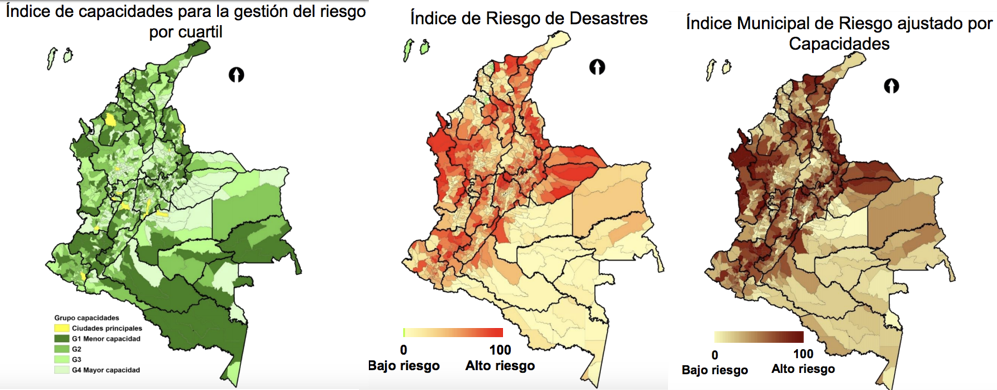
\includegraphics[width=0.95\textwidth]
        {riskIndexesCol}}
        \caption{Risk Management Index of Colombia adjusted on the basis of capacities. The index which is illustrated on the right image combines the capacity of territorial subdivisions to manage the risk (image on the left), and their risk of a disaster (image in the center). Image taken from \cite{XX}}
        \label{fig:riskIndex}
      \end{figure}
      

%%%IMPORTANTE AFTER 2012
%Acciones 2012: 
%Modernizo su sstema nacional de gestion de riesgo. 
%Politica nacional de gestion de riesgo de desastres

%2010 y 2016 se invirio en gestion del riesgo de dsstres 3 veces mas que en el periodo 2002  y 2009 esa inversion se concentra a nivel nacional y municipal BAJO departamental

